This is a very important section, you explain to us how you made it work.

\subsection{Theoretical Background}
If you are using theoretical concepts, explain them first in this subsection.
Even if they come from the course (e.g., lattices), try to explain the essential
points \emph{in your own words}. Cite any reference work you used like this
\cite{TigerBook}. This should convince us that you know the theory behind what
you coded.

\subsection{Implementation Details}

We make use of some properties of the KOOL language to make the implementation simple:

\begin{itemize}
    \item All classes are declared the the top level
    \item All methods are declared at the top level of a class
    \item The language has no inclusion or import feature
\end{itemize}

These properties allow for easy lookup of templates, since for example there is no need to search
for template declarations in statements. This makes the implementation easy --- in fact, class
templates can be completely expanded as a separate phase before name analysis since the name lookup
in this case is so simple. Method template expansion is done as part of the type checking phase,
since we need to know the receiver type of a method call before we can look up the method template.

Since templates may reference themselves or other templates, template expansion is done iteratively.
The class template expansion phase loops back to itself if any templates were expanded, and the
method template expansion subphase loops back to class template expansion if any templates were
expanded. \figref{compiler-flowchart} illustrates the flow between compiler phases.

\begin{figure}[hbtp]
  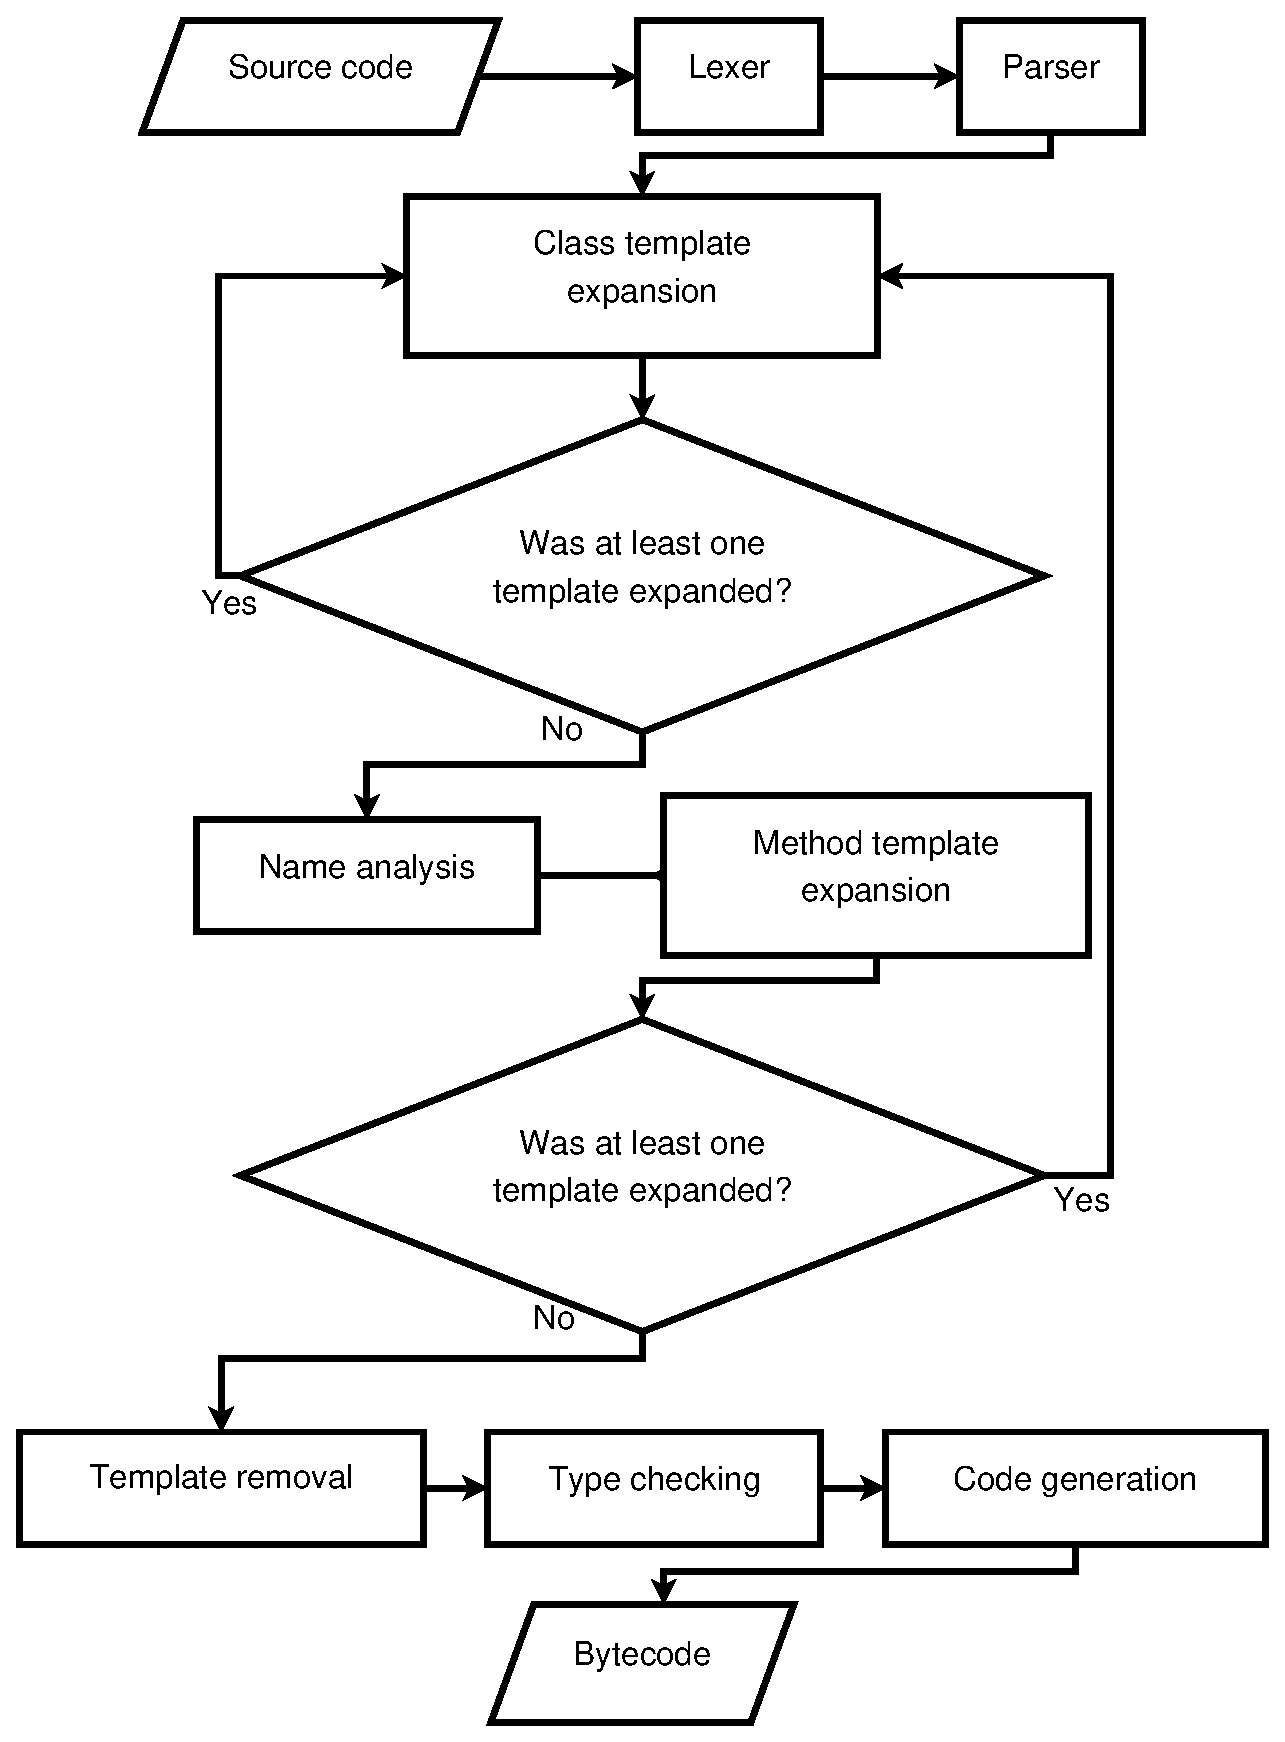
\includegraphics[width=0.5\textwidth]{compiler-flowchart}
  \caption{Compiler phases flow diagram. Since templates may reference other templates that may in
    turn need expansion, the template expansion phases must be iterated until all template
    references have been replaced with references to concrete expanded types or methods.}
  \label{fig:compiler-flowchart}
\end{figure}

In each iteration of the template expansion phases, only the leaves in each tree of template
parameters is expanded.


\emph{Describe all non-obvious tricks you used. Tell us what you thought was hard and
why. If it took you time to figure out the solution to a problem, it probably
means it wasn't easy and you should definitely describe the solution in details
here. If you used what you think is a cool algorithm for some problem, tell us.
Do not however spend time describing trivial things (we know what a tree traversal
is, for instance).}

\emph{After reading this section, we should be convinced that you knew what you were
doing when you wrote your extension, and that you put some extra consideration
for the harder parts.}
